\section{Source Coding}
\lecture{11 Mar.}

\subsection{Shannon's Source Coding Theorem}
In Shannon's 1948 paper, he introduced source coding as a mean of compression for a source, i.e., a sequence of symbols $X_i$. The information theorist Blahut further defines \textit{compression} as \textit{lossy compression}, and \textit{compaction} as \textit{lossless compression}.

The following information quantity is useful in describing source coding:
\begin{definition}[Entropy]
    For an i.i.d. source $X$ following a probability density function (can be easily extended to the continuous case) $p(x)$, we define its entropy to be
    \begin{equation}
        H(X) = -\sum_{x}p(x)\lg p(x) \text{ bits.}
    \end{equation}
    If $\ln$ is used in place of $\lg$, the units changes from ``bits'' to ``nats''.
\end{definition}
\begin{theorem}[Shannon's Source Coding Theorem]
    Given an i.i.d. source $X_1$, $X_2$, $\ldots$, a total of $H(X)+\varepsilon$ bits are needed per observation to describe the source.
\end{theorem}
\begin{example}
    Consider the following \textit{Huffman coding}, which is an easier version of Shannon's source coding theorem. Let a random source of nucleobases $X$ be equal to $A$ w.p. $\frac{1}{2}$, $C$ w.p. $\frac{1}{4}$, $G$ w.p. $\frac{1}{8}$, or $T$ w.p. $\frac{1}{8}$. Since $-\lg p(A) = 1$, we should use 1 bit to describe $A$; since $-\lg p(C) = 2$, we should use 2 bits to describe $C$; and similarly, we should use 3 bits to describe both $G$ and $T$. For example, we encode the nucleobases by $A:0$, $C:10$, $G:110$, and $T:111$. If one tries to encode $n$ nucleobases, we have the total expected bits used as
    \begin{equation*}
        \frac{n}{2}\cdot1 + \frac{n}{4}\cdot2 + \frac{n}{8}\cdot 3 + \frac{n}{8}\cdot3 = \frac{7}{4}n \text{ bits} = n\cdot H(X).
    \end{equation*}
\end{example}

Let us define a few more terms:
\begin{definition}[Information Density]
    We define the information density / surprisal of a realization $x$ of the random variable $X$ as
    \begin{equation}
        h(x) = -\lg p(x).
    \end{equation}
    Entropy is equal to the expected surprisal, i.e., $H(X) = \mathbb{E}[h(X)]$.
\end{definition}
\begin{definition}[Asymptotic Equipartition Property, AEP]
    This describes the log version of the law of large number. Notice that
    \begin{equation}
        h(x_1\ldots x_n) = -\lg\left(p(x_1)\cdots p(x_n)\right) = \sum_{i=1}^n -\lg p(x_i) = \sum_{i=1}^n h(x_i).
    \end{equation}
    This is an i.i.d. sum of R.V.s! We can use the concentration inequality:
    \begin{equation*}
        \mathrm{Pr}\left\{\frac{\sum_{i=1}^n h(X_i)}{n} - H(X) \ge \varepsilon\right\} \le \exp(-c\varepsilon^2n).
    \end{equation*}
    The AEP property simply states the concentration of the average of information density converges to the entropy.
\end{definition}
Let us now prove the theorem. We will further use polar code to achieve it. 
\begin{proof}[Proof. (Shannon's Source Coding Theorem, fixed length version)]
    Let us try to encode as many length $n$ strings as possible using only $n\left(H(X)+2\varepsilon\right)$ bits. Let us define a \textit{typical set}
    \begin{equation}
        \mathcal{A}(\varepsilon) \defeq \setdef{x_1\ldots x_n \in \mathcal{X}^n}{h(x_1\ldots x_n) \le n\left(H(X)+\varepsilon\right)}.
    \end{equation}
    For a string $x_1\ldots x_n\in\mathcal{A}(\varepsilon)$, we have
    \begin{equation}
        p(x_1\ldots x_n) \ge 2^{-n\left(H(X)+\varepsilon\right)} \Rightarrow \abs{\mathcal{A}(\varepsilon)} \le 2^{n\left(H(X)+\varepsilon\right)}.
    \end{equation}
    Thus, the set $\mathcal{A}(\varepsilon)$ can be mapped injectively onto bit string of length $n\left(H(X)+\varepsilon\right)$. What about the sequences outside of $\mathcal{A}(\varepsilon)$? Luckily, by the concentration inequality, their total probability of appearing is exponentially small and can be neglected.
\end{proof}
\begin{proof}[Proof. (Shannon's Source Coding Theorem, variable length version)]
    If fix length encoding fails to describe a source, we can use the suboptimal ``literal'' encoding for some strings. An encoding of a string either looks to have around $n H(X)$ bits for those in $\mathcal{A}(\varepsilon)$, or that they are described by $Cn$ bits, where $C$ is a constant. Then the expected value of the code length will be
    \begin{align*}
        \mathbb{E}[\text{length}] = \left(1-\exp(-c\varepsilon^2n)\right) \cdot n\left(H(X)+\varepsilon\right) + \exp(-c\varepsilon^2n)\cdot Cn = n\left(H(X)+2\varepsilon\right).
    \end{align*}
\end{proof}

In fact, most of our modern day coding uses variable length coding, as one can easily check that photos saved in your phone album has varying file size.

\subsection{Arithmetic Encoding}
\begin{example}
    Consider a source $X$ being equal to $A$ w.p. $\frac{2}{3}$, equal to $C$ w.p. $\frac{1}{3}$. Then given a string, for example $ACAACAC$, we can encode it into a binary string by the following procedure:
    \begin{figure}[H]
        \centering
        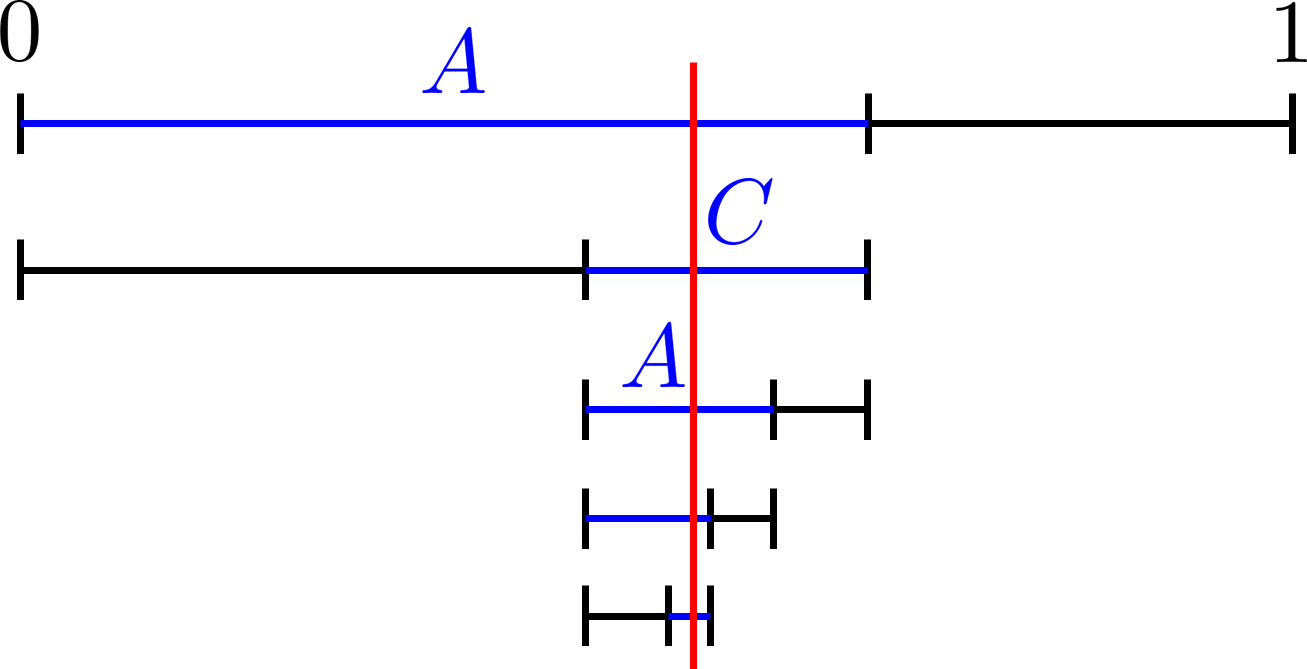
\includegraphics[width=0.5\linewidth]{figures/w4_arithmetic_encoding.png}
        \caption{Illustration of arithmetic encoding.}
    \end{figure}
    By continuing partitioning the interval with respect to the probability one can find a shortest binary string in the last interval and use it to represent the original string of symbols. In our case above, the last interval is $[124/243,44/81]\approx[0.510288,0.543209]$, the shortest bit string within is $0.10001$ in binary. The number of bits needed is approximately
    \begin{align*}
        \lg\frac{1}{\text{smallest interval size}} &= \lg\left(\frac{2}{3}\cdot\frac{1}{3}\cdot\frac{2}{3}\cdot\frac{2}{3}\cdot\frac{1}{3}\cdot\frac{2}{3}\cdot\frac{1}{3}\right)^{-1} \\
        &= -\lg\left(\prod p(x_i)\right)\\
        &\approx -\lg\left.2^{nH(X)}\right|_{n=7} = n H(X)\approx 6.4.
    \end{align*}
\end{example}
Note that arithmetic encoding is in fact capacity-achieving as seen in the example above. However, due to patent reasons, this code is not widely used.

\subsection{Source Coding with Incorrect Code}
Suppose that we have a coding scheme designed specifically for $\mathrm{Ber}(q)$. However, if the true underlying distribution is $\mathrm{Ber}(p)$ where $q\neq p$, what will happen?

Obviously, the compression to the code would not be as good as initially expected. In fact, we can characterize the extra length to the code paid by our ignorance to be
\begin{align*}
    \mathbb{E}_{\mathrm{Ber}(p)}\left[-\lg q(X)\right] - \mathbb{E}_{\mathrm{Ber}(p)}\left[-\lg p(X)\right] &= \left[-p\lg q - (1-p)\lg(1-q)\right] \\
    &\;\;\;\;\;\;- \left[-p\lg p - (1-p)\lg(1-p)\right] \\
    &= p\lg\frac{p}{q} + (1-p)\lg\frac{1-p}{1-q} \\
    &\eqdef D_{\mathrm{KL}}(P\mid\mid Q).
\end{align*}
The term $D_{\mathrm{KL}}$ that we obtained here is another important information theoretical quantity:
\begin{definition}[Kullback-Leibler Divergence, KL Divergence]
    For two distributions $P$ and $Q$, we can define their KL divergence to be
    \begin{equation}
        D_\mathrm{KL}(P\mid\mid Q) \defeq \mathbb{E}_{P}\left[\lg\frac{P}{Q}\right] = \sum p_i \lg\frac{p_i}{q_i}.
    \end{equation}
\end{definition}
It is easy to see that the KL divergence must be greater than or equal to zero. Moreover, given $D_{\mathrm{KL}}(P\mid\mid Q)$, it describes the expected surprise from modeling as $Q$ given the true underlying distribution being $P$.

\subsection{Source Polarization}
For source coding, there are three different methods: Shannon's source coding theorem, arithmetic encoding, and Ar{\i}kan's source polarization. We have talked about the previous two already, let us discuss how the polarization trick we have seen earlier from noisy-channel coding can also be used in source coding. Note that the following trick we introduce has great advantage when we want to apply it to distribution shaping in the future.

In essence, source polarization is equivalent to channel polarization but without looking at the channel outputs. Given two symbols $U_1$, $U_2$ in a field $F$. Then, let us consider a similar scheme as in channel polarization:
\begin{enumerate}
    \item What is the distribution of $X_1\defeq U_1+U_2$?
    \item Given $U_1+U_2$, what is the distribution of $X_2\defeq U_2$?
    \item Do the same polarization recursion: given two copies of $U$ from the same distribution, construct $X_1$ and $X_2$ as $U^+$ and $U^-$. Given two copies of $U^+$, construct $U^{++}$ and $U^{+-}$; given two copies of $U^-$, construct $U^{-+}$ and $U^{--}$. And so on.
\end{enumerate}
One should be able to observe that $H(U^{\pm\pm\ldots})$ polarizes to 0 or $\lg\abs{F}$, which corresponds to a constant random variable or a uniform distribution over $F$, respectively.

The number of $s\in\{+,-\}^n$ such that $H(U^s)\approx 0$ is about $2^n(1-\frac{H(U)}{\lg\abs{F}})$; the number of $s\in\{+,-\}^n$ such that $H(U^s)\approx \lg\abs{F}$ is about $2^n(\frac{H(U)}{\lg\abs{F}})$. By a similar argument using martingale, the quantity going up or down remains balanced so as to have the expectation unchanged. We do not provide a detailed proof here.

The source coding scheme under this setup is: remember those $U^s$ that satisfy $H(U^s) \approx \lg\abs{F}$, i.e., remember those that are random. This scheme is, in fact, capacity-achieving.

Amazingly, polar code can do both source coding and noisy-channel coding as defined by Shannon's 1948 paper.


\subsection{Source Coding with Side Information} \label{sec:slepian_wolf_1}
Given a source that generates a pair of random variables $(X_i,Y_i)$ where $X_i$ is what one tries to remember, and $Y_i$ is the \textit{side information} available at both the encoder and decoder.
\begin{figure}[H]
    \centering
    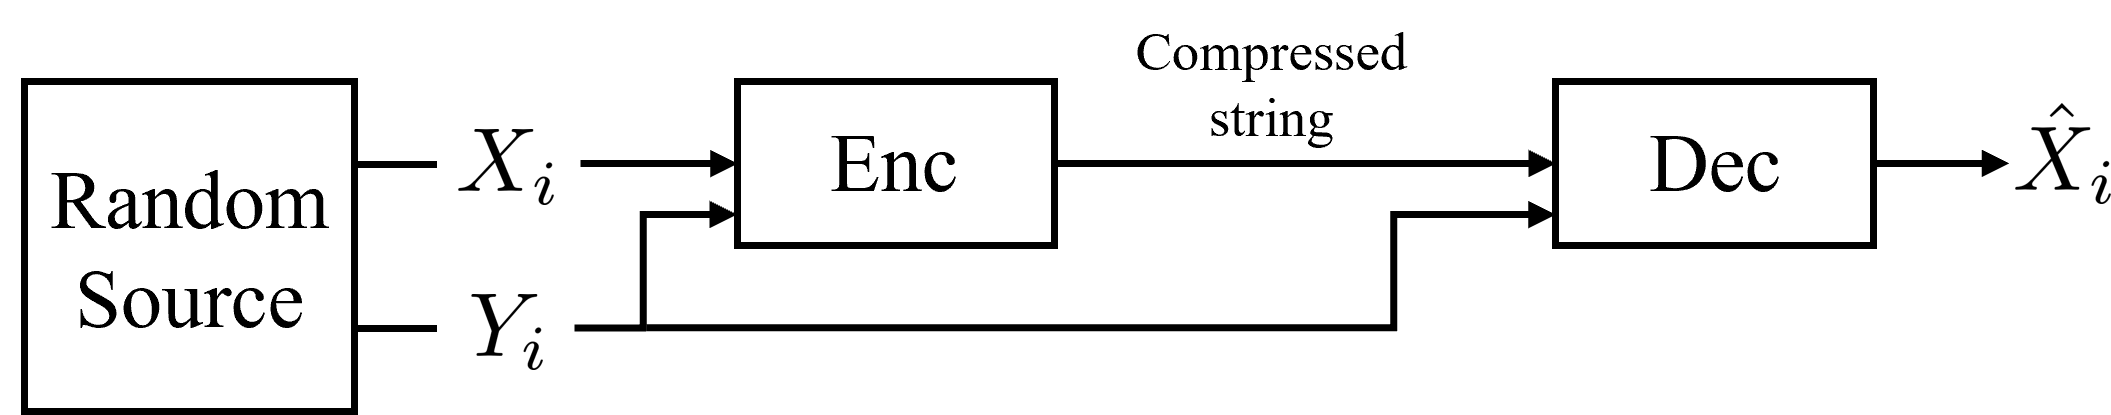
\includegraphics[width=0.8\linewidth]{figures/w4_enc_dec.png}
    \caption{Illustration of source coding with side information.}
\end{figure}
The code rate is the \textit{conditional entropy} $H(X\vert Y) = H(X,Y) = H(Y)$, which satisfies $H(X\vert Y)\le H(X)$. This is the Slepian-Wolf coding, developed after WWII to figure out the amount of information needed to be sent from spy planes with overlapping scanning areas.

The proof to the Slepian-Wolf coding as a valid coding method is similar to that as Shannon's source coding theorem:
\begin{enumerate}
    \item Define conditional information density $h(x_i\vert y_i) = -\lg p(x_i\vert y_i)$.
    \item $h(x_1\ldots x_n\vert y_1\ldots y_n) = $ sum of i.i.d. R.V.s $ = \sum_i h(x_i\vert y_i)$.
    \item $\mathcal{A}(\varepsilon) = \setdef{\text{string}}{h\le n(H(X\vert Y)+\varepsilon)}$. (AEP and typical set)
    \item Find injection between $\mathcal{A}(\varepsilon)$ and strings of length $n(H(X\vert Y)+\varepsilon)$.
    \item Bound error probability by concentration inequality.
\end{enumerate}

Similarly, one can realize the capacity-achieving property using polar code. The proof is also of similar fashion:
\begin{enumerate}
    \item Define polarized random variables $(X\vert Y)^\pm$.
    \item Check for polarization: $H((X\vert Y)^s)=0$ or $\lg\abs{F}$.
    \item Find number of $s$ such that $H$ is high is about $2^n(H(X\vert Y)+\varepsilon)$.
    \item Remember these random variables that are almost uniformly random.
    \item Check for capacity-achieving property.
\end{enumerate}

